%%report template for pattern recognition SS2016

\documentclass[english, paper=a4]{scrartcl}
\usepackage[utf8]{inputenc}
% images
\usepackage{graphicx}
%math
\usepackage{amsmath,amssymb}
%code
\usepackage{algorithm}
\usepackage[noend]{algpseudocode}
\makeatletter
\def\BState{\State\hskip-\ALG@thistlm}
\makeatother

\usepackage{subcaption}
\captionsetup{compatibility=false}
\usepackage{multirow}
\usepackage{color}
\usepackage{enumitem}
\usepackage{float}
\usepackage{listings}

\DeclareMathOperator*{\argmax}{arg\,max} 

\begin{document}

\graphicspath{{images/}}


%%------------------------------------------------------
%% provide your input here:
\title{Bayesian Network Inference with Cuda} 

\subtitle{GPU Architecture} 

\author{Christian Brändle (1428543), Marc Haubenstock (1525175)}



%%------------------------------------------------------

\maketitle

\section{Hidden Markov Model(HMM)}

\subsection{Overview}



Signals are often thought of as the product of sources that act statistically.
Our goal is to model these statistical properties. Our basis of model building depends on 
assumptions about liminations in the model's degree of freedom. 
Further the model should deliver useful information for segmenting signals into meaningful units
\cite{mm_pr}[p.71]

A \emph{Hidden Markov Model} describe a \textbf{two-state stochastic process} \cite{mm_pr}[p.72].
There is a stochastic process that is stationary (which means its probabilistic features don't change over time) and a \emph{state space} that is finite.
A \emph{Markov Chain Model} probabilistically describes the state transitions as a \emph{finite state automaton} - see table \ref{tab:FiniteSA}.

% figure for state transition table as finite state automaton
\begin{table}[h]
	\begin{center}
		\begin{tabular}{| c | c |}
			\hline
			\multicolumn{2}{|l|}{
				\begin{tabular}{ l }
					\emph{Finite state automatons} \\
				\end{tabular}
			} \\
			\hline
			& \\
			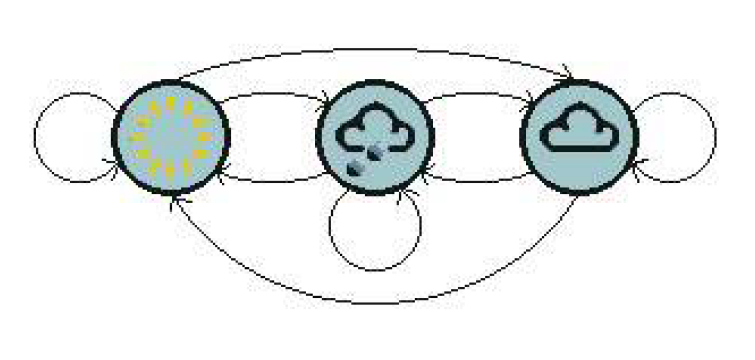
\includegraphics[width=0.33\textwidth]{./Images/FiniteStateAutomaton_1.png} & 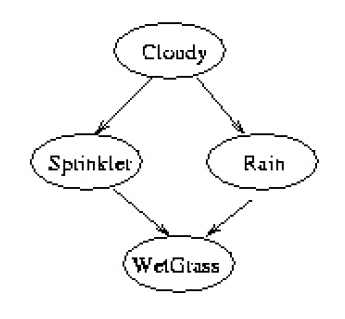
\includegraphics[width=0.33\textwidth]{./Images/FiniteStateAutomaton_2.png} \\
			\hline
			weather HMM \cite{hmm_fb} & grass HMM \cite{gm_bn} \\
			\hline
		\end{tabular}
	\end{center}
	\caption{Two finite state automatons that describe the state space of two different HMMs. Nodes correspond to states and edges to transition probabilites betwenn states that are bigger than $0$.}
	\label{tab:FiniteSA}
\end{table}

The important thing is that \textbf{the behaviour of the process given at time $t$ only depends on the immedate predessor state} \cite{mm_pr}[p.72]. So the \emph{Markov property} \eqref{eq:markProp} states:

\begin{equation}
	P(S_t | S_1,S_2, \ldots S_{t-1}) = P(S_t | S_{t-1})
	\label{eq:markProp}
\end{equation}

Visually this can be shown with a graph model of a HMM as a sequence of hidden states $X_i$ and the corresponding obervations $Y_i$ - see figure \ref{fig:GraphModel}.

% GraphModelHMM_1.png
\begin{figure}[H]
	\centering
	
	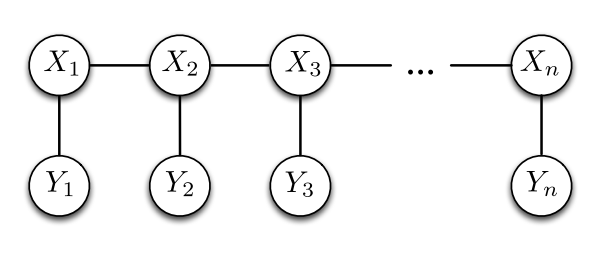
\includegraphics[width=0.66\textwidth]{./Images/GraphModelHMM_1.png}
	\caption{ \cite{hmm_II}}
	\label{fig:GraphModel}
\end{figure}

In the second stage at every point in time $t$ an output obervation $O_t$ (or $Y_t$) is generated. The corresponding \textbf{probability distribution only depend on the current state} \cite{mm_pr}[p.72]. This is called the \emph{output independence assumption} \eqref{eq:outIndep}.

\begin{equation}
P(O_t | O_1,O_2, \ldots O_{t-1}) = P(O_t | S_{t-1})
\label{eq:outIndep}
\end{equation} 

The model itself is \emph{'hidden'} because we only can observe the outputs generated, namely the \emph{observation sequence} $O_1, O_2, \ldots,  O_T$.

For initialization of the model additional start probalilities are used that describe the start probability distribution at time $t=1$.

A hidden Markov model denoted as $\lambda$ is described by \cite{mm_pr}[p.73]:

\begin{itemize}
	\item a finite set of states $S$ \\ 
	$ S = \left\{s | 1 \leq s \leq N \right\} $
	\item a state-transition probalilitiy matrix $A$ \\ 
	$A = \left\{ a_{ij} | a_{ij} = P(S_t = j | S_{t-1} = i) \right\}$
	\item a start probability vector $\Pi$ \\ 
	$ \Pi = \left\{ \Pi_i | \Pi_i = P(S_1 = i)  \right\}$
	\item specific state probability dirstibutions for the outputs of the model,  \\
	$\left\{ b_j(o_k) | b_j(o_k) = P(O_t = o_k | S_t = j) \right\}$ \\
	if observations are discrete we can write in matrix form \\
	$ B = \left\{ b_{kj} | b_{kj} = P(O_t = o_k | S_t = j) \right\} $
\end{itemize}

According to \cite{cuhmm}[p.2] the used notation of HMM elements in the paper and in the provided codes in detail corresponds to:

\begin{figure}[H]
\centering

\includegraphics[scale=0.4]{"symbols"}
  \caption{The notation of a HMM \cite{cuhmm}}
\end{figure}


\subsection{Forward}

\begin{figure}[H]

\centering
\includegraphics[scale=0.4]{"FW"}
 \caption{Pesudo-Code for the Forward Algorithm \cite{cuhmm}}

\end{figure}

The algorithm produces a data structure called a trellis, denoted by \(\alpha\) of size \(N \times T \) for a sequence of $T$ observations of size $N$. The trellis can be viewed as a matrix where each cell \(\alpha(t,i)\) holds the probability of being in state \(i\) while having seen the observations until \(t\). The complexity of the algorithm is due to the for loops. For \(M\) observation sequences the complexity of the algorithm is 
$\mathcal{O}(MN^2T)$. Due to the dependency on a previous value as shown line 7, the outer most for loop can not be parallised. Instead, we can exploit the fact that all our \(M\) observation sequences are independent, this can be computed in parallel, reduced the complexity to $\mathcal{O}(cMT)$, where $c$ is the execution time of the parallel code \cite{cuhmm}.

\subsection{Viterbi}

\begin{figure}[H]

\centering
\includegraphics[scale=0.4]{"vit"}
 \caption{Pesudo-Code for the Viterbi Algorithm \cite{cuhmm}}

\end{figure}

The goal of the viterbi algorithm is to find the most likely path in the state space of a known HMM provided a given observation sequence. The computation of the $\alpha$-trellis corresponds to that of the forward algorithm. The only difference is that instead of a summation over te probabilities associated with the predessor states a maximization is performed \cite{mm_pr}[p.86].
Because the globally optimal probability of the optimal state sequence $s^*$ is only known after the evaluation of the final $\alpha$-trellis line at time $T$ the \emph{backtrace} can only be started after the complete $\alpha$-trellis is calculated.
First the state that maximizes the corresponding element in the last line of the $\alpha$-trellis marks the point of tracing back through the tracted probabilities and descitions (i.e. state transitions) made while the $\alpha$-trellis was computed.

More formally, for all $\alpha_{t+1}(j)$ where $j$ indicates the jth state the corresponding $\gamma_{t+1}(j)$ tracking looks like equation \eqref{eq:trace}:

\begin{eqnarray}
	\forall t = 1, \ldots, T-1: \\
	\alpha_{t+1}(j) = \max_i \left\{ \alpha_{t}(i)*a_{ij} \right\} *b_j(O_{t+1})  \\
	\gamma_{t+1}(j) = \argmax_{i} \left\{ \alpha_{t}(i)*a_{ij} \right\}
	\label{eq:trace} 
\end{eqnarray}  

The corresponding backtracking looks like equation \eqref{eq:backtrack}:

\begin{eqnarray}
	P^*(O | \lambda) = P(O, s^* | \lambda) = \max_j \alpha_T(i) \\
	\forall t = T-1, \ldots, 1: \\
	s^*_t = \gamma_{t+1}(s^*_{t+1})
	\label{eq:backtrack} 
\end{eqnarray}

\subsection{Baum-Welch}


\begin{figure}[H]

\centering
\includegraphics[scale=0.4]{"BW"}
 \caption{Pesudo-Code for the Backward Forward Algorithm \cite{cuhmm}}

\end{figure}

The general structure of the Baum-Welch algorithm is similar to its forward counterpart. Most notably instead of iterating from the start of the observation sequence, the algorithm starts at the last observation, moving backwards through the trellis. The parallisation can be achieved in a similar manner to the forward algorithm, but due to the change in indexing for the trellis \(\alpha\) in line 11 this can not be repesented as matrix multiplcation \cite{cuhmm}.

The idea of this algorithm is to (randomly) initialise the A and B matrices, perform the forward, then the backward pass on them. Finally with the computed values we can re-estimate the matrices and repeat the process.

Sadly numerous errors in the pseudo code made the implementation more difficult than presented. Specifically in line 9, the probability \(p\) is produced from the transition matrix \(A\) not the trellis, as is evident from the inconsistent indexing at \(\alpha\). Moreover, at line 10. the \(\beta\) values is not dependent on \(i-1\) but rather \(i\) \cite{hmm}. 

\begin{figure}[H]

\centering
\includegraphics[scale=0.4]{"estimation"}
 \caption{Estimation of the A and B Matricies \cite{cuhmm}}

\end{figure}

Similarly the estimated values of the emission matrix B is not dependent on \(\epsilon(j)\), but should be on \(\gamma\), as it is defined in literature \cite{hmm}. 

\newpage


\section{Implementation}

\subsection{Overview}

As seen in the previous section it is not possible to fully parallize the individual algorithms due to their dependence on a value of a previous time \(t\). However, hmms are usually computed with many observation sequences \textbf{M}. Each algorithm acts on one such sequence. The main idea presented in \cite{cuhmm} exploits this by parallizing over \textbf{M} instead of \(T\). 

\begin{figure}[H]
\centering

\includegraphics[scale=0.3]{"3d_trellis"}
  \caption{Graphical representation of the data structure presented in \textit{A Cuda Implementation of Hidden Markov Models}\cite{cuhmm}}
\end{figure}


Thus, the for-loop of the T domain remains in the code while the CUDA kernel computes all M slices at time t in parallel. Graphically this can be seen as moving through the 3D data structure either front-to-back, in the forward case, or back-to-front in the backward case. The current element is being computed by applying the following formulae.

\begin{center}

\( D_{ij} = B_{O_i} .* C_i \times A_j \)

\end{center}

Where \( B_{O_i}\) is the row of the emission matrix at observation \(O_i\), \(C_i\) is the previous slice and \(A_j\) is the j\textsuperscript{th} column of the transition. matrix A.

\begin{figure}[H]
\centering

\includegraphics[scale=0.3]{"slice"}
  \caption{The computation of a slice\cite{cuhmm}}
\end{figure}

Finally a stipulation of the outlined method is that:

\begin{itemize}
\item The number of states and sequences must be a multiple of block size 16
\item The number of output sequences must be of the same length.
\end{itemize}

\subsection{Forward}
\begin{verbatim}
	initTrellis<<<M,N>>>(..);

	for(int t = 0; t < T; t++){
		...
		
		 // copute B_o
		computeBRow<<<M,N>>>
		(M_noOfObsSequences, V_noOfObsSymbols, T_noOfObservations, 
		N_noOfStates, dev_O_obsSequence_2D, dev_B_obsEmissionProbs_2D, i, dev_B);
		
		cudaDeviceSynchronize();
		
		 // W = B_o .* C_i
		pointwiseMul<<<M,N>>>
		(dev_W, dev_B, &dev_3D_Trellis[(i - 1) * M_noOfObsSequences * N_noOfStates]);
		
		cudaDeviceSynchronize();
		
				// wrapper function for cublas multiply; D = W x A
		cublasDeviceMultiply(M_noOfObsSequences, N_noOfStates, N_noOfStates, dev_W, 
		dev_A_stateTransProbs_2D, &dev_3D_Trellis[i * M_noOfObsSequences * N_noOfStates]); 

		
		cudaDeviceSynchronize();
		
		...
		
	
	}
	
	double *last_slice 
	= &dev_3D_Trellis[(T_noOfObservations - 1) * M_noOfObsSequences * N_noOfStates];	
	
	// compute likelihood
	for (int i = 0; i < M_noOfObsSequences; i++)
	{

		int smBytes = 64 * sizeof(double);
		int grid = N_noOfStates / 64;
		reduce_1 <<< grid, 64, smBytes >>>(&last_slice[i*N_noOfStates], dev_A_odata);

		memcpyVector(host_A_odata, dev_A_odata, N_noOfStates, cudaMemcpyDeviceToHost);

		host_likelihoods_1D[i] = host_A_odata[0] + host_A_odata[1];

	}

\end{verbatim}

The implementation follows the pseudo-code outlined by Liang. First we compute the slices of our 3D data structure by looping over T. Instead of only computing a single value as outlined by the eqution, we compute all values for a slice at once.Once we computed all values, we compute the likelihood for each observation sequence. No pseudo-code was given, however, by looking at literature we know we have to compute this as a summation of all terms for a single observation sequence \cite{hmm}. We implementing this summation as a reduction in \(N\). The reduction uses the simple interleaved model and is outlines as the first method in \textit{Optimizing Parallel Reduction in CUDA} \cite{reduction}.

\subsection{Viterbi}

The actual viterbi calculation of the $\alpha$-trellis and the corresponding trace $\gamma$-trellis is done within a host device method to use the same code across different CPU and GPU implementations.

\begin{lstlisting}

__host__ __device__ void viterbi1D(double *dev_Alpha_trelis_2D, 
unsigned int *dev_Gamma_trellis_backtrace_2D,...)
{
  // determine indices
  ...

  // actual calculation
  double a_ji = dev_A_stateTransProbs_2D[idx_a_ji];
  double b_it = dev_B_obsEmissionProbs_2D[idx_b_it];
  double p = a_ji * b_it;
  double alpha_tm1j = 
  dev_Alpha_trelis_2D[idx_alpha_tm1j];
  double alpha_ti = 
    dev_Alpha_trelis_2D[idx_alpha_ti];
  double partPathProb_tm1j = alpha_tm1j * p;
  if (partPathProb_tm1j >alpha_ti)
  {
    dev_Alpha_trelis_2D[idx_alpha_ti] = 
      partPathProb_tm1j;
    // backpointers(t,i) = j
    dev_Gamma_trellis_backtrace_2D[idx_alpha_ti] = 
      idx_j;
  }
}

\end{lstlisting}

In the one dimensional approach we just execute multiple instances of the viterbi algorithm in parallel on our set of oberservation sequences. So we expect linear performance improvement depending on the number of parallel executions of viterbi algorithms. Because this parallelization has the limmitation of using only one kernel per observation sequence we can only gain performance if we run a lot of observation sequences in parallel. The data transfer between CPU and GPU as well as the fact that one GPU kernel performs less Giga-FLOPS as a corresponding CPU kernel shows that this is not a well scaling form of parallelisation.
In real world situations we are not able to saturate the GPU with enough parallel execution lines.
The corresponding kernel function shows the execution for one obersation sequence, i.e. a complete viterbi run.

\begin{lstlisting}

__global__ void viterbiKernel1D(... 
int *dev_likeliestStateIndexSequence_2D)
{
  // determine matrix dimensions
  ...

  // slice matrices according to idx_m
  int idx_m = blockIdx.x * blockDim.x + threadIdx.x;

  // check if idx_m is out of range and abort this kernel thread
  if (idx_m > M_noOfObsSequences)
    return;

  double *dev_Alpha_trelis_TN_2D = 
    dev_Alpha_trelis_TNM_3D + (idx_m*dim1_Alpha*dim2_Alpha);
  int *dev_Gamma_trellis_backtrace_TN_2D = 
    dev_Gamma_trellis_backtrace_TNM_3D + 
    (idx_m*dim1_Gamma*dim2_Gamma);

  int* dev_O_obsSequence_1D = 
    dev_O_obsSequences_2D + idx_m*dim1_obsSeq;

  int* dev_likeliestStateIndexSequence_1D = 
    dev_likeliestStateIndexSequence_2D + 
    (idx_m*T_noOfObservations);
	
  // device memory initialization
  TrellisInitialization2D(dev_Alpha_trelis_TN_2D, ...);
	
  // actual calculation - creating indices for viterbi1D
  for (int idx_t = 1; idx_t < T_noOfObservations; idx_t++)
  {
    for (int idx_i = 0; idx_i < N_noOfStates; idx_i++)
    {
      for (int idx_j = 0; idx_j < N_noOfStates; idx_j++)
      {
        // calling viterbi1D
        viterbi1D(dev_Alpha_trelis_TN_2D, 
        dev_Gamma_trellis_backtrace_TN_2D, ...);
      }
    }
		
    // rescaling of Trellis' to avoid numerical problems
    TrellisScaling2D(dev_Alpha_trelis_TN_2D, ...);
  }
	
  // extract most likely path of states that generates observation
	
  // backtrace(t,i) = j;
  double partPathProb_optT = 0;
  unsigned int idx_j = 0;
  for (int idx_i = 0; idx_i < N_noOfStates; idx_i++) 
  {
    if (idx_i == 0 || 
      dev_Alpha_trelis_TN_2D[(T_noOfObservations - 1)*
      N_noOfStates + idx_i] > partPathProb_optT)
    {
      partPathProb_optT = 
        dev_Alpha_trelis_TN_2D[(T_noOfObservations - 1)*
        N_noOfStates + idx_i];
      idx_j = idx_i;
    }
  }
	
  dev_likeliestStateIndexSequence_1D[T_noOfObservations - 1] = idx_j;
  for (int idx_i = 1; idx_i < T_noOfObservations; idx_i++)
  {
    dev_likeliestStateIndexSequence_1D[T_noOfObservations - 1 - idx_i] =
    dev_Gamma_trellis_backtrace_TN_2D[(T_noOfObservations - idx_i)*
    N_noOfStates +
    dev_likeliestStateIndexSequence_1D[T_noOfObservations - idx_i]];
  }

}

\end{lstlisting}


\subsection{Baum-Welch}

\begin{verbatim}


	initMatrix<<<N_noOfStates,V_noOfObsSymbols>>>(dev_B_prime_3D,M_noOfObsSequences);
	initMatrix<<<N_noOfStates,N_noOfStates>>>(dev_A_prime_3D, M_noOfObsSequences);
	
	// overwrite the "true" transfer and emission matricies with the random ones
	copyMatrix(dev_A_prime_3D, host_A_stateTransProbs_2D,
	 N_noOfStates, N_noOfStates, M_noOfObsSequences);
	copyMatrix(dev_B_prime_3D, host_B_obsEmissionProbs_2D, 
	N_noOfStates, V_noOfObsSymbols, M_noOfObsSequences);
	
	initBeta<<<M_noOfObsSequences, N_noOfStates>>>(dev_beta_3D, V_noOfObsSymbols);
	
	ForwardAlgorithmSet(host_Pi_startProbs_1D, host_A_stateTransProbs_2D, 
	host_B_obsEmissionProbs_2D,host_O_obsSequences_2D, N_noOfStates, 
	V_noOfObsSymbols, T_noOfObservations, M_noOfObsSequences,host_likelihoods_1D...);
	
	
\end{verbatim}

The matrices and $\beta$ values are initialized and copied into host memory for the forward algorithm.
	
\begin{verbatim}
	

	for (int t = T_noOfObservations - 1; t >= 0; t--) {
	
	UpdateGammaGPU << <M_noOfObsSequences, N_noOfStates >> >
	(dev_gamma_3D, dev_beta_3D, dev_3D_Trellis_Alpha, t, dev_likelihood, V_noOfObsSymbols);

		cudaDeviceSynchronize();

		UpdateEpsilonReductionErrorGPU <<<M_noOfObsSequences, N_noOfStates >>>
		(epsilon_reduction_grid_error, dev_beta_3D, dev_3D_Trellis_Alpha, t, dev_likelihood);
		
		if (t > 0){

			// Computes the B matrix in term D = B .* C x A
			ComputeBDevice << < M_noOfObsSequences, N_noOfStates >> >
			(M_noOfObsSequences, V_noOfObsSymbols, T_noOfObservations, 
			N_noOfStates, dev_O_obsSequences_2D, dev_B_obsEmissionProbs_2D, t, dev_B);
			cudaDeviceSynchronize();

			// All dimensions are multipe of Warp Sizes
			// Compute W =  B .* C i.e. beta(t,i) * b_it
			pointwiseMatrixMul << <M_noOfObsSequences, N_noOfStates >> >
			(dev_W, dev_B, &dev_beta_3D[t * M_noOfObsSequences * N_noOfStates]);

			cudaDeviceSynchronize();

			// Compute D = W x A, D = beta(t,i)*p
			cublasMultiplyDouble(M_noOfObsSequences, 
			N_noOfStates, N_noOfStates, dev_W, dev_A_stateTransProbs_2D, dev_D);

			cudaDeviceSynchronize();

			updateBeta << <M_noOfObsSequences, N_noOfStates >> >
			(dev_beta_3D, dev_D, t, V_noOfObsSymbols);

			cudaDeviceSynchronize();


			for (int j = 0; j < N_noOfStates; j++){
				UpdateEpsilonGPU <<<M_noOfObsSequences, N_noOfStates >>>
				(dev_epsilon_3D, dev_beta_3D,
				dev_3D_Trellis_Alpha, t, dev_likelihood, j, dev_D);

				cudaStatus = cudaDeviceSynchronize();
			} // end of for j

		} // end of if
	
	} // end of for t
	
	\end{verbatim}
	
	The values presented in the pseudo code (Figure 3) at lines 6 and 7 can be computed easily as CUDA kernels. Similarly the values of \(\beta\) follow a similar procedure as the \(\alpha\) values in the forward algorithm, and can be computed accordingly. The \(\epsilon\) values on the other hand depend on 3 variables \(i,j,m\). Because of this, we opted for a simple approach and iterate over \(N\), to compute this value, increasing the complexity to $\mathcal{O}(cMNT)$.
	
		\begin{verbatim}
	
	// Estimate Matricies - 	// sum up all values and reductions then divide

	ColumReduction_Height <<<1, N_noOfStates >>>
	(epsilon_reduction_grid_error, M_noOfObsSequences);
	ColumReduction_Height <<<N_noOfStates, N_noOfStates >>>
	(dev_epsilon_3D, M_noOfObsSequences);

	ColumReduction_Height <<< N_noOfStates,V_noOfObsSymbols>>>
	(dev_gamma_3D, M_noOfObsSequences);
	ColumReductionGamma_Depth <<<1, N_noOfStates >>>
	(dev_gamma_3D, 0, V_noOfObsSymbols,M_noOfObsSequences, gamma_reduction_grid);

	EstimateA <<<N_noOfStates, N_noOfStates>>>
	(dev_A_prime_3D, dev_epsilon_3D, epsilon_reduction_grid, 
	epsilon_reduction_grid_error, 0, M_noOfObsSequences);

	EstimateB <<<V_noOfObsSymbols, N_noOfStates>>>
	(dev_B_prime_3D, dev_gamma_3D, gamma_reduction_grid, 0, M_noOfObsSequences);
\end{verbatim}

Since the formula for computing the estimate \(\hat{b}\) is incorrect we had to adopt our own approach.

\begin{figure}

\centering

\( \hat{b}_j(v_k) = \frac{\text{expected number of times in state j observing symbol } v_k}{\text{expected number of times in state j}} \)
\caption{Definition of b hat taken form \cite{hmm}}

\end{figure}

This is implemented as the reduction concerning the gamma data structures in our code. First, we compute all values of \(\gamma_t(i,j)\) by summing over \(M\), then we compute \(\gamma_t(j)\) by summing over the symbol domain \(V\), and store this in our reduction data structure.

\section{Evaluation}

\subsection{Data Generation \& Setup}

Our data generation happens in two passes. First we produce the transition and emission matrices $A$ and $B$. All values in these matrices are random, but picked such that each row sums to 1. Once the matrices have been generated we use the sequence generator of Liu \cite{hmm} to produce observation sequences of length $L = 16$. Both of these stages are performed on the CPU with regular C++ code.

To evaluate the runtime of the CUDA kernels we used NVIDIAs \textit{cudaEventRecord}. An example of how we implement this in code is as follows.

\begin{verbatim}
	startBenchmark(..);
	for (int i = 0; i < ITERATIONS; i++)
	{
		// run kernel
	}
	stopBenchmark(..);
\end{verbatim}

Where \textit{startBenchmark} and \textit{stopBenchmark} are wrapper functions for \textit{cudaEventRecord}.
To evaluate the correctness of our algorithms we compared them to the output of Lui's implementation with the same data set. However, the forward algorithm was able to be executed alone in Liu's code. Therefore we wrote our own serial implementation and compared it against that. Although this is not very precise, the algorithm is simple enough to write from scratch.

From this we can assert that our forward and viterbi algorithms produce correct results. However, the Baum-Welch algorithm does not. Clearly there is an error in the algorithm, but due to the sloppy defintion of this alorithm presented in \cite{cuhmm}, it is not clear where this error is. Nevertheless, we give our results of all algorithms in the next section.

\subsection{Comparison}

\begin{figure}[H]
\centering
\begin{tabular}{|l|l|}
\hline
GPU &GForce GTX 860M \\ \hline
CPU & intel i7-4710HQ @2.50 GHz with 8 GB of RAM  \\ \hline
OS & Windows 10 \\ \hline
CUDA & CUDA 7.5 CM 3.0 \\ \hline
Host Compiler & Visual Studio 2013 \\ \hline

\end{tabular}

\caption{Test Environment}
\end{figure}

\begin{figure}[H]
\centering
\begin{tabular}{|l|l|l|l|}
\hline
Data size (N $\times$ M) & Liu CPU & Liu GPU & GPU (Average of 1000 Iterations)\\ \hline
64 $\times$ 64 & 687.7 & 10.2 & 13.6 \\ \hline
128 $\times$ 128 & 5621.9 & 19.74 & 18.15 \\ \hline
192 $\times$ 192 & 18990.5 & 40.93 & 35.93 \\ \hline
256 $\times$ 256 & 45031.6 & 71.77 & 47.20 \\ \hline
320 $\times$ 320 & 88090.8 & 128.44 & 77.09 \\ \hline
448 $\times$ 448 & 152374.8 & 208.08 & 124.99 \\ \hline
512 $\times$ 512 & 360899.3 & 410.17 & - \\ \hline

\end{tabular}

\caption{Comparing the run time of the forward algorithm in ms}
\end{figure}

\begin{figure}[H]
\centering
\begin{tabular}{|l|l|l|}
\hline
Data size (N $\times$ M) & CPU 1D & GPU 1D \\ \hline
64 $\times$ 64 & 208.53 & 902.71 \\ \hline

\end{tabular}

\caption{Comparing the run time of the BW algorithm in ms}
\end{figure}


\begin{figure}[H]
\centering
\begin{tabular}{|l|l|l|l|}
\hline
Data size (N $\times$ M) & Liu CPU & Liu GPU & GPU + CPU(Average of 1000 Iterations)\\ \hline
64 $\times$ 64 & 2138.4 & 35.9 & 115.43 \\ \hline
128 $\times$ 128 & 7891.1.9 & 142.6 & 297.26 \\ \hline
192 $\times$ 192 & 57681.3 & 339.1 & 722.38 \\ \hline
256 $\times$ 256 & 136694.2 & 903.3 & - \\ \hline
320 $\times$ 320 & 267038.8 & 1328.6 & - \\ \hline
448 $\times$ 448 & 461297.6 & 2479.6 & - \\ \hline
512 $\times$ 512 & 1094036.4 & 6054.8 & - \\ \hline

\end{tabular}

\caption{Comparing the run time of the BW algorithm in ms}
\end{figure}

\subsection{Conclusion}

Examining figure 9. we can see that our algorithm outperforms Liu's code, however the paper was published in 2009. Therefore, it is safe to assume that our set up was using better hardware and compiler technologies than available to Liu. Nevertheless, we can see that the performance gain of the GPU code is very significant.

Most notably the measurement from the last row is missing. This is most probably due to a memory leak in our code as experiments with a low iteration count still complete.

The results for the Viterbi algorithm were very underwhelming. Although we do everything in CUDA kernels, the kernel still follows the serial structure of the pseudocode i.e. for loops. Nevertheless, we can see that, maybe not surprisingly, CUDA is not good for implementing serial code.

Therefore, for the Baum-Welch algorithm we incorporated CPU measurements into our results. The reason for this is that some work is done on the CPU side and it would falsify our measurements if we would omit this. For this reason our measurements are much larger than Liu's pure GPU performance. As mentioned before, our Baum-Welch implementation fails to produce correct values, however we do not believe this to be a problem of the algorithm's general structure. Therefore, the algorithms overall complexity will likely not change for a correct implementation.

As before omitted values indicate a memory leak.

In general it can be seen that by using the GPU considerable performance gains can be made when applied to Hidden Markov Models. Further improvements can be made by using Texture Memory \cite{cuhmm} as data structures such as the transition and emission matrices are read only for the forward and viterbi algorithm. Furthermore, dynamic parallelism can be use to optimize the code further, as renditions can be spawned form inside CUDA kernels and thus don't require context switching back to the CPU. These could be topics for future projects.



%%------------------------------------------------------



\bibliographystyle{plain}
\bibliography{HMM}
%% References can be stored in a seperate bib-file (see lit.bib). References, that are cited in the report using \cite are automatically added to the reference list. For more information: http://www.bibtex.org/Using/
%%------------------------------------------------------
\newpage

\section{Appendix}
\subsection{CUDA Kernels}

\begin{verbatim}
// FROM: NVIDIA Optimizing Parallel Reduction in CUDA
__global__ void reduce_1(double* g_idata, double* g_odata){

	extern __shared__ double sdata[];

	unsigned int tid = threadIdx.x;
	unsigned int i = blockIdx.x*blockDim.x + threadIdx.x;

	sdata[tid] = g_idata[i];

	__syncthreads();

	for (unsigned int s = 1; s < blockDim.x; s *= 2){
		if (tid % (2 * s) == 0){
			sdata[tid] += sdata[tid + s];
		}

		__syncthreads();
	}

	if (tid == 0){
		g_odata[blockIdx.x] = sdata[0];
	}
}
\end{verbatim}

\begin{verbatim}
__global__ void pointwiseMatrixMul(double * dev_w, double *dev_A, double* dev_B){

	unsigned int ix = blockIdx.x * blockDim.x + threadIdx.x;

	unsigned int idx_k = ix;

	dev_w[idx_k] = dev_A[idx_k] * dev_B[idx_k];

}
\end{verbatim}

\begin{verbatim}
__global__ void AlphaTrellisInitializationGPU(double *dev_3D_Trellis, const double *dev_Pi_startProbs_1D, const double *dev_B_obsEmissionProbs_2D, const unsigned int *dev_O_obsSequences_2D, int T_noOfObservations, int N_noOfStates, int V_noOfObsSymbols){

	int obs_index = blockIdx.x * T_noOfObservations;
	int obs_start = dev_O_obsSequences_2D[obs_index];
	int idx_b_i_idxOs = threadIdx.x*V_noOfObsSymbols + obs_start;
	int idx_alpha_0i = blockIdx.x * N_noOfStates + threadIdx.x;
	int idx_pi_i = threadIdx.x;

	double alpha_0_i 
	= dev_Pi_startProbs_1D[idx_pi_i] * dev_B_obsEmissionProbs_2D[idx_b_i_idxOs];
	dev_3D_Trellis[idx_alpha_0i] = alpha_0_i;


}
\end{verbatim}

\begin{verbatim}
__global__ void initMatrix(double* matrix_3D, int depth){

			int idx_3D = threadIdx.x*gridDim.x*depth + blockIdx.x;

			matrix_3D[idx_3D] = 1.0f / blockDim.x;

}
\end{verbatim}

\begin{verbatim}
__global__ void initBeta(double* beta_3D, int T_noOfObservations){

	// 2D index
	int idx = blockIdx.x*blockDim.x + threadIdx.x;

	int offset = gridDim.x*blockDim.x*(T_noOfObservations - 1);

	beta_3D[offset + idx] = 1;

}

__global__ void updateBeta(double* dev_beta_3D, double* dev_D, 
int t, int T_noOfObservations){

	int idx_2D = blockIdx.x*blockDim.x + threadIdx.x;
	int idx_t_minus_1 = (t - 1)*blockDim.x*gridDim.x + idx_2D;


	dev_beta_3D[idx_t_minus_1] += dev_D[idx_2D];
}

__global__ void EstimateB(double* dev_update, double*dev_source,
 double* reduction_grid, int m, int M){

	int idx_3D = m * blockDim.x + blockIdx.x*blockDim.x*M + threadIdx.x;
	int idx_top = blockIdx.x*blockDim.x*M + threadIdx.x;

	int reduction_idx = threadIdx.x;

	double val = dev_source[idx_top];
	dev_update[idx_top] = val / reduction_grid[reduction_idx];

}

__global__ void EstimateA(double* dev_update, double*dev_source,
 double* reduction_grid, double* reduction_grid_error, int m, int M){

	int idx_3D = m*blockDim.x + blockIdx.x*blockDim.x*M + threadIdx.x;
	int idx_top = blockIdx.x*blockDim.x*M + threadIdx.x;

	int reduction_idx = m*blockDim.x + blockIdx.x;
	int reduction_idx_1D = blockIdx.x;

	double val = dev_source[idx_top];
	dev_update[idx_top] = val / (reduction_grid_error[reduction_idx_1D]);


}

__global__ void ColumReduction_Height(double* dev_update, int M){

	int start = threadIdx.x + blockIdx.x*M*blockDim.x;


	for (int i = 1; i < M; i++){

		int idx = start + i*blockDim.x;

		dev_update[start] += dev_update[idx];

	}



}

__global__ void ColumReductionGamma(double* dev_update, int m, int M){

	int start = threadIdx.x + blockIdx.x*blockDim.x*M;

	for (int i = 1; i < M; i++){

		int idx = start + i*blockDim.x;

		dev_update[start] += dev_update[idx];

	}



}

__global__ void ColumReductionGamma_Depth(double* dev_update, int m,
 int V,int M, double* grid){

	int start = threadIdx.x;
	
	for (int i = 0; i < V; i++){

		int idx = start + i*blockDim.x*M;

		grid[threadIdx.x] += dev_update[idx];

	}

}
\end{verbatim}

\end{document}
